\documentclass{chem6155problemset}
\usepackage{chemfig}
\usepackage{enumitem}

\title{CHEM6155 -- Problem Set 1\\Math Foundations, Isotopes, Mathematica}
\date{DUE: FRIDAY of Week 3}



\begin{document}

\maketitle

\section{Mathematical Foundations}
The following problems are roughly aligned with the indicated chapters of Steiner, The Chemistry
Maths Book, 2nd Edition, Oxford University Press 2008. If you have difficulty with any
of these problems, please read the corresponding chapter. If that is not sufficient
to help you solve it, please contact one of the module instructors for help. Some of the problems
require you to use \emph{Mathematica}, which is available to Students from the University.
Install a copy of it on your computer. To get started, there are many tutorials and videos
available online. \emph{Mathematica} is highly complex, and like most powerful tools requires
patience and practice to master. If you run into problems, seek help from the module instructors.

\paragraph{1.1 Functions, Differentiation, and Integration}
\begin{enumerate}
 	\item Define the following properties of functions $y=f(x)$, and provide an example for each. You
	may have to look up the definitions; if so, provide the source.
	  \begin{itemize}
	  	\item monotonic
		\item bounded
		\item divergent
		\item continuous
		\item differentiable
		\item periodic
	  \end{itemize}

	 \item Indicate which of the above properties the following functions satisfy (state
	 your reasoning):
	 	\begin{itemize}
			\item $f(x)=x^2\,e^{-x}$
			\item $f(x)=\tan(1/x)$
			\item $f(x)=\cos\frac{2\pi x}{L} + 2 \sin\frac{6\pi x}{L}$
			\item $f(x) = x^3-4x^2-11x+30$
			\item $f(x) = \dfrac{x^3-4x^2-11x+30}{x^3-6}$
		\end{itemize}

	\item Plot the above functions using \emph{Mathematica}. Indicate the approximate
	positions of roots, stationary points and poles in the plots.

	\item Find the exact locations of the stationary points in these functions.
	Try to verify your answers using \emph{Mathematica}. You may need to use
	the derivative function \verb@D[f[x],x]@ and the equation solver \verb@Solve[f[x]==0,x]@


	\item Evaluate the definite integral (you may assume $R_2>0$:
		\[\displaystyle\int\limits_{0}^{\infty} e^{-i\omega t} \, e^{(i\omega_0-R_2) t}\,\mathrm{d}t\]



	 \item Plot the real and imaginary parts of  $e^{(i\omega_0-R_2) t}$
   as a function of $t$ for specific values of $\omega_0$ and $R_2$
   with \emph{Mathematica}. What does a 3D plot (complex plane vs time)
   of this curve look like?


	 \item In NMR spectroscopy, resonance lines often take the shape of the absorption mode Lorentzian function
	 \[\displaystyle g(\omega) = \frac{1}{\pi} \frac{T}{1+T^2(\omega-\omega_0)^2}\]
	 \begin{itemize}
	  \item Plot this function for various choices of the parameters $T$ and $\omega_0$. What
	 	role do these parameters play?
	  \item Find the integral $\int_{-\infty}^\infty\,g(\omega)\,\mathrm{d}\omega$ as a
	  function of the parameters $\omega_0$ and $T$. Comment on your finding.
	  \end{itemize}
\end{enumerate}

\paragraph{1.2 Algebraic Equations and Complex Numbers}

\begin{enumerate}[resume]
	\item Provide brief explanations for the following terms and expressions ($z$ is a complex number)
	\begin{itemize}
		\item complex conjugate, $z^\ast$
		\item modulus, $|z|$
		\item argument, $\arg z$
	\end{itemize}

	\item find all complex solutions to the following equations:
	\begin{itemize}
	 	\item $z^5 + 1 = 0$
		\item $z^3+2z^2+3z = 0$
		\item $\cos\frac{2\pi z}{L} + \frac{i}{2} =0$
	\end{itemize}
      \item Plot the locations of the following complex numbers in the complex plane, and compute their
	conjugate, modulus, and arguments:
	\begin{itemize}
	  \item $\exp(\pi i)$
	  \item $1+\pi i$
	  \item $\exp(\frac{\pi}{2}i)$
	  \item $1+\frac{1}{i}$
	  \item $\exp(2+\frac{\pi}{4}i)$
	  \item $\frac{1}{1-3i}$
	  \item $\frac{\sqrt{2}}{2}(1+i)$
	\end{itemize}
\end{enumerate}

\paragraph{1.3 Trigonometric Functions and Euler's Formula}
\begin{enumerate}[resume]
%  \item The two vectors $\mathbf{a}=(1,-2,0)^T$ and $\mathbf{b}=(2,1,-1)^T$ span
%    plane a $P$ in 3D space, which contains the point $(1,0,0)$. Find
%    the equation that describes the plane $P$ in the form $Ax+By+Cz+D=0$, i.e., determine
%    the coefficients $A,B,C$, and $D$.

\item Prove the following identities. You may need to use Euler's formula, $\exp i\phi = \cos\phi + i \sin\phi$.
	\begin{itemize}
		\item $\sin(\alpha\pm\beta) = \sin\alpha\cos\beta \pm \sin\beta\cos\alpha$
    \item $\cos(\alpha\pm\beta) = \cos\alpha\cos\beta \mp \sin\beta\sin\alpha$
		\item $\cos i\beta = \cosh\beta$
		\item $\sin i\beta = -i \sinh\beta$
		\item $\sin\frac{\alpha}{2}\cos\frac\alpha{2} = \frac{1}{2}\sin\alpha$
		\item $\sin(\alpha\pm i\beta) = \sin\alpha\cosh\beta \mp i \sinh\beta\cos\alpha$
		\item $\sin\frac{k\pi x}{a}\sin\frac{l\pi x}{a} = \cos\frac{(k-l)\pi x}{a} - \cos\frac{(k+l)\pi x}{a}$
	\end{itemize}

\end{enumerate}

\paragraph{1.4 Operators and Hilbert Spaces}
\begin{enumerate}[resume]
	\item Over the space of functions $f(x)$ defined on the interval $x\in [-\pi,\pi]$ a scalar
	product $\braket{f}{g}$ is defined as
	\[ \braket f g = \int\limits_{-\pi}^{\pi} f(x)^\ast \,g(x)\,\mathrm{d}x, \]
	where the asterisk marks the complex conjugate.
	Compute the scalar products of all pairs of the following functions:

	\begin{itemize}
		\item $\sin x$
		\item $\cos^2 x$
		\item $\exp(i \omega )$

	\end{itemize}

	\item A linear operator $\hat O$ maps any function $f(x)$ onto another one $g(x)$:
	\[ \hat O : f(x)\longrightarrow g(x) \]
	Linearity means that
	\[ \hat O (f(x)+g(x)) = \hat O f(x) + \hat O g(x) \quad \forall f(x),g(x). \]
	Which of the following transformations represent linear operators?
	\begin{itemize}
	  \item $f(x) \longrightarrow f(2x) $
	  \item $f(x) \longrightarrow 2f(x) $
	  \item $f(x) \longrightarrow f'(x) + f''(x)$
	  \item $f(x) \longrightarrow (f'(x))^2 $
	  \item $f(x) \longrightarrow \int_0^x\,f(u)\,\mathrm{d}u $
	\end{itemize}


	\item The stationary wave functions of a particle trapped in an infinitely deep rectangular potential
	well between $x=0$ and $x=a$ are given by
	\[ \phi_k(x) = \sqrt\frac{2}{a} \sin \frac{k \pi x}{a},\qquad k\in 1,2,\dots\]
	\begin{itemize}
		\item Verify that these wave functions are properly normalised, i.e., that $\braket{\phi_k}{\phi_l} = \delta_{kl}$
    \item Find the matrix elements $\bra{\phi_k}\hat A\ket{\phi_l}$ for the operator
    \[\hat A = \begin{cases}
         1, x<\frac{a}{2} \\
         0, \text{otherwise}
       \end{cases}
       \]

		\item Find the matrix  elements $\bra{\phi_k}\hat x\ket{\phi_l}$ of the position operator $\hat{x} = x$
      for $k,l=1\dots3$

		\end{itemize}

\end{enumerate}

\paragraph{1.4 Linear Equation Systems, Matrices and Eigenvalue Problems}

\begin{enumerate}[resume]
	\item Find all solutions $(x,y,z)$ of the equation system
	\[ \begin{array}{ccc} 3 x + 6 y -3 z = 0 \\
	   					  2 x +   y + 5z = 0 \\
						  x   +  2y - z  = 0
       \end{array}
       \]


  \item Given the following definitions, where $b, c_x, c_y, c_x,$ and $d$ are real numbers,
  \[  A=\begin{pmatrix} i \\ 2 \\ 3 \end{pmatrix}  \quad
      B=\begin{pmatrix} 0 \\ b \\ -\sqrt{3} \end{pmatrix} \quad
      C=\begin{pmatrix} 0  & -c_z &  c_y \\ c_z & 0 & -c_x \\ -c_y & c_x & 0 \end{pmatrix} \quad
      D=\begin{pmatrix} 1  & d &  1/d \\ d & -3 & 0 \\  1/d & 0 & 2 \end{pmatrix}
  \]
  evaluate the matrix products
     \begin{itemize}
        \item $AB^\dagger$
        \item $A^\dagger B$
        \item $CA$
        \item $B^\dagger C$
        \item $C^2$
        \item $C^\dagger D C$
     \end{itemize}
	\item Consider four orthonormal quantum states $\ket 1 \dots \ket 4$, and two operators $\hat A$ and $\hat B$ acting on them. These operators interchange the quantum states as indicated by the bent arrows below.

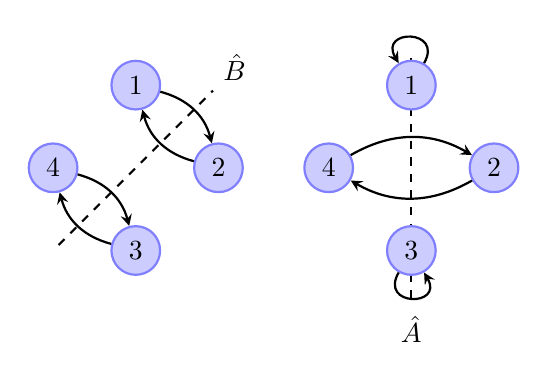
\begin{tikzpicture}[place/.style={circle,draw=blue!50,fill=blue!20,thick},>=stealth,scale=0.7]

	\draw[dashed,thick] (-1.4,-1.4) -- (1.4,1.4) node[anchor=south west] {$\hat B$};

	\node[place] (1) at (0,1.5) {$\ket 1$} ;
	\node[place] (2) at (1.5,0) {$\ket 2$} ;
	\node[place] (3) at (0,-1.5) {$\ket 3$} ;
	\node[place] (4) at (-1.5,0) {$\ket 4$} ;

	\draw[->,bend left,thick] (1) to (2) ;
	\draw[->,bend left,thick] (2) to (1) ;
	\draw[->,bend left,thick] (3) to (4) ;
	\draw[->,bend left,thick] (4) to (3) ;

	\begin{scope}[shift={(5,0)}]

		\draw[dashed,thick] (0,2) -- (0,-2.5) node[anchor=north] {$\hat A$};
		\node[place] (1) at (0,1.5) {$\ket 1$} ;
		\node[place] (2) at (1.5,0) {$\ket 2$} ;
		\node[place] (3) at (0,-1.5) {$\ket 3$} ;
		\node[place] (4) at (-1.5,0) {$\ket 4$} ;

		\draw[->,bend left,thick] (4) to (2) ;
		\draw[->,bend left,thick] (2) to (4) ;
		\draw[->,out=60,in=120,loop,looseness=4,thick] (1) to (1) ;
		\draw[->,out=240,in=300,loop,looseness=4,thick] (3) to (3) ;
	\end{scope}



\end{tikzpicture}

	\begin{enumerate}
		\item Express $\hat A$ and $\hat B$ as a superposition of $\ket n \bra m$ operators.
		\begin{solution}
			\[
				\hat A = \ket1\bra1+\ket2\bra4+\ket4\bra2+\ket3\bra3.
			\]
			\[
				\hat B = \ket1\bra2+\ket2\bra1 + \ket3\bra4+\ket4\bra3.
			\]

		\end{solution}
		\item Find their matrix representations in the basis $\ket 1 \dots \ket 4$.
		\begin{solution}
		\[
			(\hat A) = \begin{pmatrix}
				1 & 0 & 0 & 0 \\
				0 & 0 & 0 & 1 \\
				0 & 0 & 1 & 0 \\
				0 & 1 & 0 & 0
			\end{pmatrix}
		\]
		\[
			(\hat B) = \begin{pmatrix}
			0 & 1 & 0 & 0  \\
			1 & 0 & 0 & 0  \\
			0 & 0 & 0 & 1 \\
			0 & 0 & 1 & 0
			\end{pmatrix}
		\]
		\end{solution}

		\item Find an example of an eigenstate for each of the two operators $\hat A$ and $\hat B$. What are the associated eigenvalues?
		\begin{solution}
		$\ket 1$ is an eigenstate of $\hat A$, to the eigenvalue 1:
			\[ \hat A \ket 1 = \ket 1\]

		$\frac{1}{2}\left(\ket 1 + \ket 2 + \ket 3 + \ket 4\right)$ is an eigenstate of $\hat B$, with eigenvalue 1:
		\[
		 \hat B \frac{1}{2}\left(\ket 1 + \ket 2 + \ket 3 + \ket 4\right) = \frac{1}{2}\left(\ket 2 + \ket 1 + \ket 4 + \ket 3\right)
		\]
		NB: it is also an eigenstate of $\hat A$:
		\[
		 \hat A \frac{1}{2}\left(\ket 1 + \ket 2 + \ket 3 + \ket 4\right) = \frac{1}{2}\left(\ket 1 + \ket 4 + \ket 3 + \ket 2\right)
		\]
		\end{solution}

		\item Find a $\ket n\bra m$ representation for the product operator $\hat A\hat B$. In a diagram similar to the one above, explain what $\hat A\hat B$ does.
		\begin{solution} [PS]
			\[
				\hat A\hat B = (\ket1\bra1+\ket2\bra4+\ket4\bra2+\ket3\bra3)(\ket1\bra2+\ket2\bra1 + \ket3\bra4+\ket4\bra3)
			\]
			\[
				= \ket1\bra2+\ket2\bra3+\ket4\bra1+\ket3\bra4.
			\]

			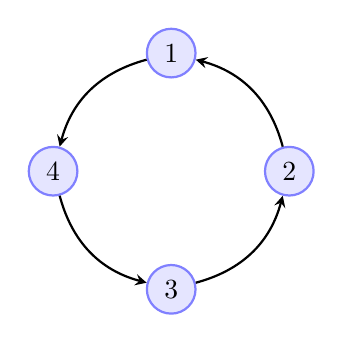
\begin{tikzpicture}[place/.style={circle,draw=blue!50,fill=blue!10,thick},>=stealth]
				\node[place] (1) at (0,1.5) {$\ket 1$} ;
				\node[place] (2) at (1.5,0) {$\ket 2$} ;
				\node[place] (3) at (0,-1.5) {$\ket 3$} ;
				\node[place] (4) at (-1.5,0) {$\ket 4$} ;

				\draw[->,bend right,thick] (2) to (1) ;
				\draw[->,bend right,thick] (3) to (2) ;
				\draw[->,bend right,thick] (1) to (4) ;
				\draw[->,bend right,thick] (4) to (3) ;
			\end{tikzpicture}


		\end{solution}

		\item 	What are the eigenvalues and eigenstates of $\hat A \hat B$?

	\end{enumerate}


	\item Assuming $A$ is an $m\times n$ matrix, and $B$ is an $n\times l$ matrix, prove
	that $(AB)^\dagger = B^\dagger A^\dagger$, where $A^\dagger$ is the conjugate transpose of $A$.

	\item Prove the following theorem: \newline
	  \emph{ All eigenvalues of a square, self-adjoint matrix $A=A^\dagger$ are real.}



\end{enumerate}


\section{Isotopes and Larmor Precession}
\paragraph{Isotopomers of Ethanol}
	Ethanol (\chemfig{CH_3CH_2OH}) consists of the elements carbon, oxygen, and hydrogen.
	\begin{enumerate}
	\item How many distinct stable (non-radioactive) isotopologues of ethanol exist?
	\item Create a table of all isotopomers of ethanol with the sum formula
	 \chemfig{^{12}C_2\, ^2H_3\, ^1H_3\,^{18}O}. Indicate which of these (if any) are chiral.
	\item Calculate the natural abundances of all possible hydrogen isotopologues of ethanol, assuming
	that the carbons are  all \chemfig{^{12}C} and the oxygen is \chemfig{^{18}O}.
	\end{enumerate}


\paragraph{Larmor Precession}
   \begin{enumerate}[resume]
   		\item What are the nuclear Larmor frequencies of \chemfig{^1H}, \chemfig{^2H},
		\chemfig{^{13}C},
		and \chemfig{^{29}Si}
		\begin{enumerate}
			\item in an NMR spectrometer operating at a magnetic field of 7T?
			\item in the earth's magnetic field?
		\end{enumerate}
   \end{enumerate}


\end{document}
